\documentclass[11pt,a4paper]{article}

\usepackage[margin=2.5cm]{geometry}
\usepackage{amsmath,amssymb}
\usepackage{graphicx}
\usepackage{booktabs}
\usepackage[round,authoryear]{natbib}
\usepackage[colorlinks=true,linkcolor=blue!50!black,citecolor=blue!50!black,urlcolor=blue!50!black]{hyperref}
\usepackage{xcolor}

\graphicspath{{../../figures/}}

\newcommand{\cl}{\mathrm{cl}}
\newcommand{\dchi}{\Delta\chi^2}

\title{Planck constraints on photon-coupled compact clumps\\ as dark matter: profile-likelihood results}
\author{S\textperiodcentered HARDY\textperiodcentered HOC\textperiodcentered PER\textperiodcentered CLAVDIVM\textperiodcentered FIERI\textperiodcentered IVSSIT}
\date{Draft of 26 September 2026}

\begin{document}
\maketitle

\begin{abstract}
We report the first real-data constraint from this project on the momentum coupling between the cosmic microwave background (CMB) photons and a population of compact, pressureless clumps that make up all of the dark matter. The coupling is expressed through the dimensionless interaction strength $u$ used by the \textsc{class} Boltzmann code, which maps directly onto the clump cross-section per unit mass and hence onto a minimum clump surface density. Profiling the likelihood over the six standard cosmological parameters and all instrumental and foreground nuisance parameters, the Planck 2018 temperature and polarization data give $u < 1.00\times10^{-4}$ at 95\% confidence, equivalent to $\sigma/M < 3.7\times10^{-7}\,\mathrm{cm^2\,g^{-1}}$ and a clump surface density $\Sigma/Q > 2.7\times10^{6}\,\mathrm{g\,cm^{-2}}$, where $Q$ is an order-unity momentum-transfer efficiency. The independent Planck PR4 (NPIPE) CamSpec high-$\ell$ likelihood gives a limit 17\% weaker, $u < 1.17\times10^{-4}$. At zero coupling the pipeline reproduces Planck's own $\Lambda$CDM fit, and the limits agree with a Fisher forecast made before any data were used. A Bayesian analysis with Markov chain Monte Carlo sampling is under way and will be added to this report.
\end{abstract}

\section{The question}
\label{sec:question}

The project asks a conditional question. If a fraction $f_\cl$ of the dark matter were in compact, pressureless clumps of ordinary matter that exchange momentum with the radiation field through an effective cross-section $\sigma$, how large could the cross-section per unit mass $\sigma/M$ be before the CMB anisotropies record the interaction? Whether such clumps can form, survive and be reconciled with Big Bang nucleosynthesis is a separate question about the premise, which we set aside here. A longer explainer covering the physics from first principles accompanies this report; the present document concentrates on the likelihood analysis and its result.

Following \citet{StadlerBoehm2018} and the interacting dark matter module of \textsc{class} \citep{Lesgourgues2011,Becker2021}, the interaction is described by
\begin{equation}
u = \frac{\sigma}{\sigma_T}\left(\frac{M}{100\,\mathrm{GeV}}\right)^{-1}
\quad\Longleftrightarrow\quad
\frac{\sigma}{M} = \frac{u}{268}\;\mathrm{cm^2\,g^{-1}},
\end{equation}
where $\sigma_T$ is the Thomson cross-section. For optically thick clumps the momentum-transfer cross-section is geometric, $\sigma = Q\,\pi R^2$, with $Q=1$ for a perfect absorber and a value of order unity for other reflection laws, so an upper limit on $u$ becomes a lower limit on the clump surface density,
\begin{equation}
\frac{\Sigma}{Q} = \frac{M}{Q\,\pi R^2} = \frac{268}{u}\;\mathrm{g\,cm^{-2}} .
\end{equation}
The coupling drags the clumps along with the radiation before recombination, which suppresses the growth of their density perturbations on small scales. The CMB sees this through the weaker gravitational potentials in the damping tail and, most strongly, through the reduced gravitational lensing of the CMB by intervening structure. The photons themselves scatter off the clumps far too rarely to matter at the couplings probed here, which is why the result does not depend on the detailed angular law of the photon--clump interaction. All results in this report assume $f_\cl = 1$ and a cross-section independent of temperature.

The same calculation has a history in particle cosmology, where the dark matter is a weakly interacting particle that scatters photons. \citet{Wilkinson2014} obtained the first Planck constraint with a modified version of \textsc{class}, finding $\sigma < 8\times10^{-31}(m/\mathrm{GeV})\,\mathrm{cm^2}$ at 68\% confidence, or $u \lesssim 1.2\times10^{-4}$, from the 2013 data. \citet{StadlerBoehm2018} repeated the analysis for the 2015 release with a more complete treatment of the photon Boltzmann hierarchy, and \citet{Zhou2022} used the 2018 release in a model in which the dark matter mass is also free. The step from particles to macroscopic objects was taken by \citet{Jacobs2015}, who proposed that the dark matter might consist of objects of gram-scale mass or more with geometric cross-sections, and who applied the bound of \citet{Wilkinson2014} to them as $\sigma_X/M_X < 4.5\times10^{-7}\,\mathrm{cm^2\,g^{-1}}$. Later studies of such objects concentrated on other effects: \citet{Caloni2021} found that for objects made of ordinary matter the strongest cosmological bound comes from the capture of baryons between nucleosynthesis and recombination, and a recent compilation of constraints as a function of the fraction of dark matter in macroscopic form \citep{Picker2026} leaves out the cosmological scattering bounds altogether as a topic to revisit. As far as we are aware, the present work is the first dedicated likelihood analysis of the photon coupling for optically thick clumps, including a check that the bound does not depend on the angular law of the photon--clump interaction.

\section{Data and method}
\label{sec:method}

\subsection{Likelihoods}

We use the Planck likelihoods as distributed through the Cobaya framework \citep{TorradoLewis2021}. Every combination includes the 2018 low-$\ell$ temperature likelihood (Commander, $2\le\ell<30$) and the low-$\ell$ E-mode polarization likelihood (SimAll), which together constrain the optical depth to reionization \citep{Planck2018V}. To these we add one of three high-$\ell$ temperature and polarization likelihoods ($\ell \ge 30$, TT, TE and EE):
\begin{itemize}
\item the 2018 \textsc{plik} likelihood, Planck's baseline, with 21 foreground and calibration nuisance parameters \citep{Planck2018V};
\item \textsc{plik}-lite, a compressed version of the same data in which the foregrounds have been marginalised in advance, leaving a single calibration parameter;
\item the PR4 (NPIPE) CamSpec likelihood \citep{Rosenberg2022}, built from the final Planck processing with a different treatment of foregrounds and sky masks, and 9 nuisance parameters.
\end{itemize}
We do not yet include the Planck lensing reconstruction likelihood, which measures the lensing potential directly from the four-point function of the maps. The lensing information used here is only that contained in the smoothing of the acoustic peaks in the power spectra.

\subsection{Theory calculation}

The CMB spectra are computed with \textsc{class} version~3.4.0, in which the clumps are the interacting dark matter species with density $\omega_{\rm idm} = f_\cl\,\omega_{\rm dm}$, a temperature-independent cross-section and a particle mass of $10^{27}$\,eV, which makes their thermal velocities negligible. Early tests showed that the default numerical settings mistreat the interaction at the couplings of interest, so we use a four times finer thermodynamics table, start the perturbation integration ten times earlier, and sample the multipoles more finely than the default in order to remove a sporadic interpolation artefact. The cosmological parameters varied are $\omega_b$, $\omega_{\rm dm}$, the angular sound horizon $100\,\theta_s$, $n_s$, $\ln(10^{10}A_s)$ and $\tau$, with one massive neutrino of 0.06\,eV as in the Planck baseline.

\subsection{Profile likelihood}

For each of eight fixed values of $u$ between 0 and $4\times10^{-4}$, we minimise $-\ln P$, the negative log posterior, over the six cosmological parameters and all free nuisance parameters, and form
\begin{equation}
\dchi(u) = 2\left[\min_{\theta}\left(-\ln P(u,\theta)\right) - \min_{u,\theta}\left(-\ln P(u,\theta)\right)\right].
\end{equation}
The only priors are Planck's own Gaussian priors on some nuisance parameters, which are the same at every $u$ and therefore cancel in $\dchi$ except through the fit. Two \textsc{plik} nuisance parameters, the thermal Sunyaev--Zel'dovich--CIB correlation and the kinetic SZ amplitude, sit at their physical lower bound of zero and were pinned there, because the minimiser otherwise wasted most of its evaluations outside the allowed range. This leaves 25 free parameters for \textsc{plik}, 15 for CamSpec and 7 for \textsc{plik}-lite.

The physical coupling cannot be negative, so the null hypothesis $u=0$ lies on the boundary of the parameter space. In that situation $\dchi$ is distributed under the null as an equal mixture of a point mass at zero and a $\chi^2$ with one degree of freedom \citep{Chernoff1954}, and the one-sided 95\% upper limit is the value of $u$ at which $\dchi = 2.71$. We quote this as the headline number and also give the crossing of $\dchi = 3.84$, which is the conventional two-sided level.

A practical difficulty is that the likelihood computed through \textsc{class} is not a perfectly smooth function of the parameters. Changing a parameter moves the internal integration and sampling grids, which produces a small, irregular noise in $-\ln P$ of about 0.03 for \textsc{plik} and 0.1--0.2 for CamSpec. Standard trust-region minimisers stop early in such a landscape and scatter by around 0.5 in $-\ln P$ between restarts, which is too much when a $\dchi$ precision of order 0.1 is needed. We therefore wrote a minimiser that samples the posterior at several hundred random points around the current estimate, fits a quadratic surface to them by least squares, moves to the fitted minimum and repeats until the predicted improvement falls below 0.01. Averaging over many points suppresses the noise, and the regression provides both the minimum value and its statistical uncertainty. The profile computations ran on a 180-core cloud machine at roughly nine likelihood evaluations per second, with each point requiring between two and five thousand evaluations.

\section{Validation}
\label{sec:validation}

At $u=0$ the model reduces to $\Lambda$CDM and the minimisation can be compared directly with Planck's published best fit. For the full \textsc{plik} likelihood we obtain $\chi^2_{\rm plik} = 2344.89$, against 2344.94 at Planck's best fit \citep{Planck2018VI}, whose fit also included the lensing reconstruction. The best-fitting parameters, $\omega_b = 0.02233$, $\omega_{\rm dm} = 0.1203$, $n_s = 0.9639$, $\tau = 0.0541$, $H_0 = 67.21\,\mathrm{km\,s^{-1}\,Mpc^{-1}}$ and $\sigma_8 = 0.812$, agree with Planck's to well within their uncertainties. The full and lite \textsc{plik} likelihoods give $\dchi$ values that agree to within 1.5\% at every $u$, which shows that pre-marginalising the foregrounds does not bias this model. Finally, a Fisher forecast made earlier in the project, with a Planck-like noise model and the six cosmological parameters free, predicted a 95\% limit of $u < 1.1\times10^{-4}$, close to what the data give.

\section{Results}
\label{sec:results}

\begin{table}[t]
\centering
\caption{Profile $\dchi(u)$ for Planck 2018 low-$\ell$ TT and EE combined with each high-$\ell$ likelihood, with $f_\cl = 1$. The statistical uncertainty of each entry from the minimisation is about 0.05 for \textsc{plik} and 0.1 for CamSpec.}
\label{tab:profile}
\begin{tabular}{lccc}
\toprule
$u$ & \textsc{plik} & \textsc{plik}-lite & PR4 CamSpec \\
\midrule
0 & 0 & 0 & 0 \\
$2\times10^{-5}$ & 0.55 & 0.56 & 0.42 \\
$5\times10^{-5}$ & 1.34 & 1.36 & 1.05 \\
$1\times10^{-4}$ & 2.71 & 2.76 & 2.18 \\
$1.5\times10^{-4}$ & 4.23 & 4.30 & 3.74 \\
$2\times10^{-4}$ & 5.94 & 6.04 & 5.27 \\
$3\times10^{-4}$ & 10.03 & 10.18 & 8.83 \\
$4\times10^{-4}$ & 15.18 & 15.34 & 13.18 \\
\bottomrule
\end{tabular}
\end{table}

\begin{figure}[t]
\centering
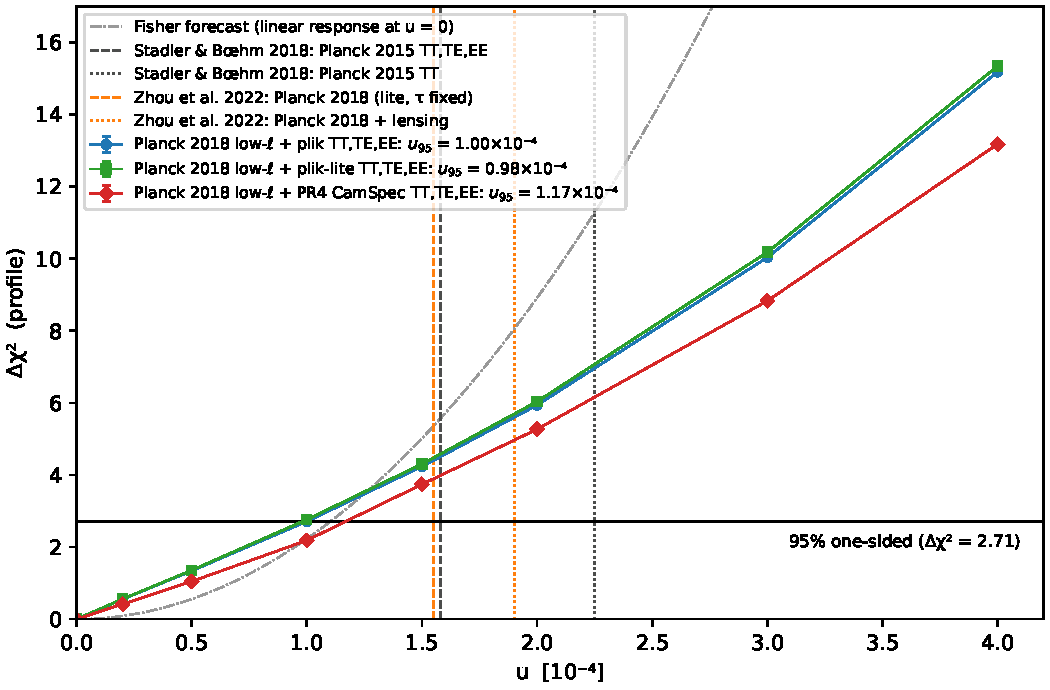
\includegraphics[width=0.9\textwidth]{report_profiles.pdf}
\caption{Profile likelihood in the clump--photon coupling $u$ for the three likelihood combinations, with all cosmological and nuisance parameters minimised at each point. The horizontal line marks the one-sided 95\% level. The vertical lines are the published marginalised 95\% limits of \citet{StadlerBoehm2018} from the Planck 2015 data (grey) and of \citet{Zhou2022} from the Planck 2018 data without and with the lensing reconstruction (orange), and the dash-dotted curve is the Fisher forecast, which assumes that the spectra respond linearly to $u$ about $u = 0$.}
\label{fig:profiles}
\end{figure}

\begin{table}[t]
\centering
\caption{Upper limits on the coupling and the corresponding clump properties for $f_\cl = 1$.}
\label{tab:limits}
\begin{tabular}{lcccc}
\toprule
High-$\ell$ likelihood & $u_{95}$ & $u(\dchi=3.84)$ & $\sigma/M$ [cm$^2$\,g$^{-1}$] & $\Sigma/Q$ [g\,cm$^{-2}$] \\
\midrule
\textsc{plik} (baseline) & $1.00\times10^{-4}$ & $1.37\times10^{-4}$ & $<3.7\times10^{-7}$ & $>2.7\times10^{6}$ \\
\textsc{plik}-lite & $0.98\times10^{-4}$ & $1.35\times10^{-4}$ & $<3.7\times10^{-7}$ & $>2.7\times10^{6}$ \\
PR4 CamSpec & $1.17\times10^{-4}$ & $1.53\times10^{-4}$ & $<4.4\times10^{-7}$ & $>2.3\times10^{6}$ \\
\bottomrule
\end{tabular}
\end{table}

Table~\ref{tab:profile} and Figure~\ref{fig:profiles} show the profiles. In every case the best fit lies at $u = 0$ and $\dchi$ rises steadily with the coupling. With the baseline \textsc{plik} likelihood the 95\% upper limit is
\begin{equation}
u < 1.00\times10^{-4}, \qquad \frac{\sigma}{M} < 3.7\times10^{-7}\,\mathrm{cm^2\,g^{-1}}, \qquad \frac{\Sigma}{Q} > 2.7\times10^{6}\,\mathrm{g\,cm^{-2}} ,
\end{equation}
and Table~\ref{tab:limits} collects the corresponding numbers for the other likelihoods. For scale, a surface density of $3\times10^{6}\,\mathrm{g\,cm^{-2}}$ is that of a column of rock about ten kilometres long, so the CMB alone allows clumps that are very dense by astronomical standards but not extreme ones. Figure~\ref{fig:limits} places these limits alongside the forecasts and the published bounds.

Figure~\ref{fig:limits} includes two sets of published limits. \citet{StadlerBoehm2018} analysed the 2015 Planck release and found $u < 1.58\times10^{-4}$ from temperature and polarization and $u < 2.25\times10^{-4}$ from temperature alone. Our limit is about 35\% tighter than the first of these. Part of the difference could come from the better polarization data and revised treatment of large-scale polarization in the 2018 release, but a larger part is probably statistical in origin, because their limits are Bayesian marginalised limits while ours come from a profile. When the parameter has a physical boundary at zero and the likelihood is not Gaussian in it, the two kinds of limit need not coincide, because the marginalised limit integrates the posterior mass above $u$, including the volume of the other parameters that remains compatible with the data, while the profile records only the best fit at each $u$. The most recent published limit, from \citet{Zhou2022}, uses the same 2018 release and gives $u < 1.55\times10^{-4}$, also as a marginalised Bayesian limit. It is not a like-for-like comparison either, since that analysis uses the \textsc{plik}-lite likelihood, holds the optical depth fixed at $\tau = 0.054$, and varies a dark matter mass in the keV--MeV range that gives the dark matter a small pressure, but it shows that with the same data the marginalised limit lies well above our profile limit. The Bayesian analysis described in Section~\ref{sec:mcmc} will allow a like-for-like comparison with our own pipeline.

\begin{figure}[t]
\centering
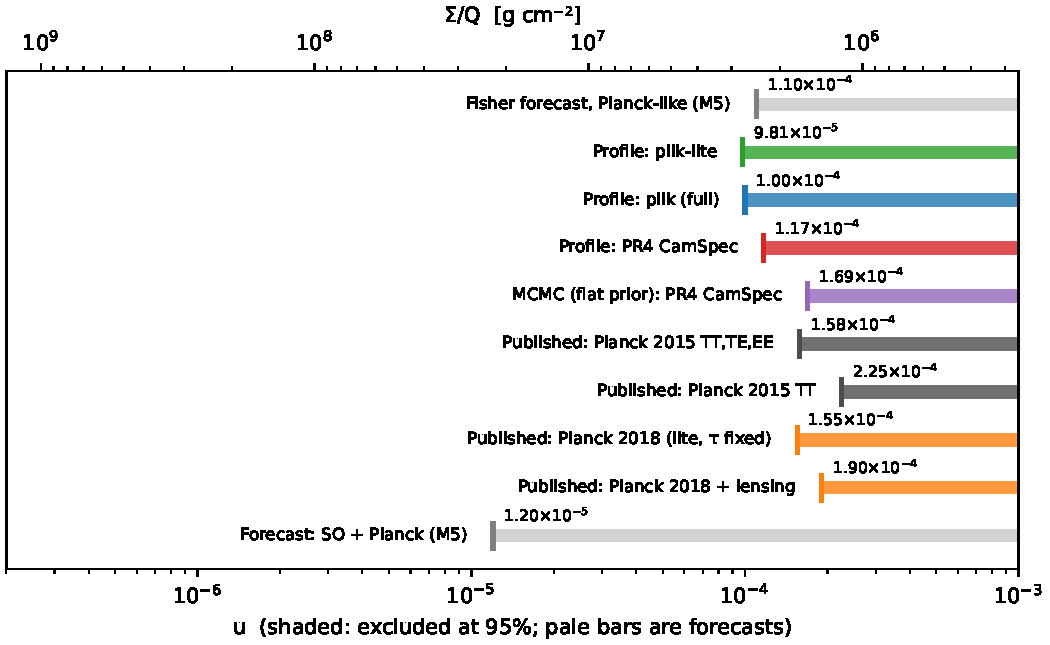
\includegraphics[width=0.9\textwidth]{report_limits.pdf}
\caption{Summary of the 95\% upper limits on $u$, with the equivalent minimum clump surface density on the upper axis. Shaded bars mark the excluded region. The pale bars are forecasts: the Planck-like Fisher forecast made before the data were used, and the forecast for Simons Observatory combined with Planck, which would improve the limit by nearly an order of magnitude.}
\label{fig:limits}
\end{figure}

\section{How robust is the result?}
\label{sec:robustness}

Several features of the analysis give us confidence in the headline number. The pipeline reproduces Planck's $\Lambda$CDM fit to 0.05 in $\chi^2$, the compressed and full \textsc{plik} likelihoods agree, the Fisher forecast agrees, and two independent high-$\ell$ likelihoods built from different processing of the Planck maps give limits within 20\% of each other. The numerical noise in the minimisation corresponds to an uncertainty of about 0.05 in $\dchi$ for \textsc{plik}, or roughly 2\% in the limit, and about twice that for CamSpec. For two of the CamSpec points ($u = 1.5$ and $2\times10^{-4}$) the final regression was noisier than the iterations that preceded it and was rejected in favour of the last converged iteration; these points lie on a smooth curve with their neighbours, but they deserve a repeat run if the CamSpec number is to be quoted to better than 10\%.

The shape of the profile deserves comment. If the spectra responded linearly to $u$ and the data were exactly those of the best-fitting $\Lambda$CDM model, $\dchi$ would rise quadratically, as the Fisher curve in Figure~\ref{fig:profiles} does. Instead it rises almost linearly from $u = 0$ and becomes gradually steeper. Two effects can produce this. The first is that the response of the spectra to $u$ is sublinear, which was already noticed in the Fisher calculation, where the derived sensitivity changed by a few per cent with the size of the finite-difference step. The second is that the data prefer the direction opposite to the one in which $u$ pushes the model, which is to say towards more lensing than $\Lambda$CDM predicts. The Planck 2018 spectra are known to show such a preference, with a phenomenological lensing amplitude $A_L = 1.18 \pm 0.07$ where unity is expected \citep{Planck2018VI}, while the PR4 CamSpec spectra show a much weaker one, $A_L \approx 1.04$ \citep{Rosenberg2022}. The initial slope of the CamSpec profile is about 20\% lower than that of \textsc{plik}, which is what the second explanation would lead one to expect. If this is the explanation, the \textsc{plik} limit is somewhat tighter than the sensitivity of the data would suggest, because a statistical fluctuation towards extra lensing counts against the clumps, and the CamSpec number is the more conservative of the two. Independent support for this interpretation comes from \citet{Zhou2022}, whose limit weakens from $1.55$ to $1.90\times10^{-4}$ when the Planck lensing reconstruction is added, since the reconstruction measures a lensing amplitude close to the $\Lambda$CDM value and so removes part of the pull that the power spectra exert against the coupling. A direct test would be to repeat the profile on simulated data generated from the best-fitting $\Lambda$CDM model, which isolates the sensitivity from the fluctuation, or to free $A_L$ alongside $u$.

The result also rests on assumptions that are separate from the numerics. All the dark matter is taken to be in clumps. For a smaller clumped fraction only part of the matter is dragged, so the limit on $u$ weakens, but how quickly it does so has not yet been computed with the likelihood. The Planck lensing reconstruction is not included. Lensing is the main channel through which the coupling is seen, so one might expect the reconstruction to tighten the limit, but the published analysis of \citet{Zhou2022} found the opposite, a weakening of about 20\%, for the reason discussed above. We expect a similar effect here, which would move the \textsc{plik} limit towards the CamSpec value. Finally, the analysis answers the conditional question posed in Section~\ref{sec:question}: it says what the CMB permits if clumps exist throughout the acoustic epoch, and it is silent on whether they can.

\section{Bayesian analysis (in progress)}
\label{sec:mcmc}

A Markov chain Monte Carlo analysis with the same PR4 CamSpec and low-$\ell$ likelihoods is running at the time of writing. It samples $u$ with a flat prior on $[0, 10^{-3}]$, a choice that \citet{DiacoumisWong2019} showed gives limits consistent to within 20\% with the Jeffreys prior, whereas a prior flat in $\log u$ makes the limit depend on an arbitrary lower cut-off. The six cosmological and nine nuisance parameters are sampled alongside it, using 24 independent chains whose proposal distribution is taken from the covariance measured in the profile at $u=0$, and it exploits the fact that the nuisance parameters can be varied without recomputing the CMB spectra. Convergence will be assessed with the Gelman--Rubin statistic across chains. The resulting marginalised limit on $u$, its comparison with the profile limit, and the joint posteriors of $u$ with the cosmological parameters, in particular $\omega_{\rm dm}$, $\theta_s$, $\omega_b$ and $\sigma_8$, with which it is expected to be most degenerate, will be added in this section.

\section{Summary}

Treating all of the dark matter as compact clumps coupled to the photons through a geometric cross-section, the Planck 2018 temperature and polarization spectra require the coupling to satisfy $u < 1.0\times10^{-4}$ at 95\% confidence, or equivalently a clump surface density $\Sigma/Q > 2.7\times10^{6}\,\mathrm{g\,cm^{-2}}$. The final Planck processing gives a limit 17\% weaker, and the difference between the two likelihoods is consistent with the known difference in their preference for extra lensing. The limit agrees with an advance forecast and is tighter than the published marginalised limits from the 2015 and 2018 data, as a profile limit on a parameter with a physical boundary is expected to be. The application of the particle bound to macroscopic dark matter was first made by \citet{Jacobs2015}; what this analysis adds is a dedicated treatment of opaque clumps with current likelihoods. The main open items are the Bayesian limit, a test of how much the Planck lensing excess tightens the bound, and the extension to populations in which only part of the dark matter is clumped.

\begin{thebibliography}{99}

\bibitem[Becker et~al.(2021)]{Becker2021}
Becker N., Hooper D.~C., Kahlhoefer F., Lesgourgues J., Sch\"oneberg N., 2021, \emph{Cosmological constraints on multi-interacting dark matter}, JCAP 02, 019.

\bibitem[Caloni et~al.(2021)]{Caloni2021}
Caloni L., Gerbino M., Lattanzi M., 2021, \emph{Updated cosmological constraints on macroscopic dark matter}, JCAP 07, 027.

\bibitem[Chernoff(1954)]{Chernoff1954}
Chernoff H., 1954, \emph{On the distribution of the likelihood ratio}, Ann.\ Math.\ Stat.\ 25, 573.

\bibitem[Diacoumis \& Wong(2019)]{DiacoumisWong2019}
Diacoumis J.~A.~D., Wong Y.~Y.~Y., 2019, \emph{On the prior dependence of cosmological constraints on some dark matter interactions}, JCAP 05, 025.

\bibitem[Jacobs et~al.(2015)]{Jacobs2015}
Jacobs D.~M., Starkman G.~D., Lynn B.~W., 2015, \emph{Macro dark matter}, MNRAS 450, 3418.

\bibitem[Lesgourgues(2011)]{Lesgourgues2011}
Lesgourgues J., 2011, \emph{The Cosmic Linear Anisotropy Solving System (CLASS) I: overview}, arXiv:1104.2932.

\bibitem[Picker et~al.(2026)]{Picker2026}
Picker Z.~S.~C., Buchanan A., Diamond M., Bramante J., 2026, \emph{Macroscopic dark matter constraints for extended mass functions}, arXiv:2609.05626.

\bibitem[Planck Collaboration(2020a)]{Planck2018V}
Planck Collaboration (Aghanim N. et~al.), 2020a, \emph{Planck 2018 results. V. CMB power spectra and likelihoods}, A\&A 641, A5.

\bibitem[Planck Collaboration(2020b)]{Planck2018VI}
Planck Collaboration (Aghanim N. et~al.), 2020b, \emph{Planck 2018 results. VI. Cosmological parameters}, A\&A 641, A6.

\bibitem[Rosenberg et~al.(2022)]{Rosenberg2022}
Rosenberg E., Gratton S., Efstathiou G., 2022, \emph{CMB power spectra and cosmological parameters from Planck PR4 with CamSpec}, MNRAS 517, 4620.

\bibitem[Stadler \& Boehm(2018)]{StadlerBoehm2018}
Stadler J., Boehm C., 2018, \emph{Constraints on $\gamma$-CDM interactions matching the Planck data precision}, JCAP 10, 009.

\bibitem[Torrado \& Lewis(2021)]{TorradoLewis2021}
Torrado J., Lewis A., 2021, \emph{Cobaya: code for Bayesian analysis of hierarchical physical models}, JCAP 05, 057.

\bibitem[Wilkinson et~al.(2014)]{Wilkinson2014}
Wilkinson R.~J., Lesgourgues J., Boehm C., 2014, \emph{Using the CMB angular power spectrum to study dark matter--photon interactions}, JCAP 04, 026.

\bibitem[Zhou et~al.(2022)]{Zhou2022}
Zhou Z., Liu G., Mu Y., Xu L., 2022, \emph{Limit on the dark matter mass from its interaction with photons}, Phys.\ Rev.\ D 105, 103509.

\end{thebibliography}

\end{document}
